\documentclass{standalone}
\usepackage{pgfplots}
\begin{document}
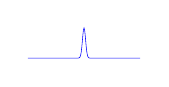
\begin{tikzpicture}[scale=.5]
\pgfplotsset{width=5cm,height=2.5cm}
\begin{axis}[axis lines=none,scaled ticks=false,mark=none]
\newcommand{\xo}{-8}
\newcommand{\xI}{8}
\addplot[blue!100!brown,domain=\xo:\xI,samples=201]{exp(-10*x^2)};
%\addplot[blue!60!brown,domain=\xo:\xI,samples=201]{exp(-10*(x-3)^2)};
%\addplot[blue!20!brown,domain=\xo:\xI,samples=201]{exp(-10*(x-6)^2)};
\end{axis}
\end{tikzpicture}
\end{document}
